\documentclass{article}
\usepackage{float}
\usepackage[pdftex]{graphicx}
\usepackage{listings}
\usepackage{xcolor}
\lstset{basicstyle=\ttfamily,
  showstringspaces=false,
  commentstyle=\color{red},
  keywordstyle=\color{blue}
}
\begin{document}

\author{Jon Robison}
\title{CS595 Assignment 6}
\maketitle

Q1. We know the result of the Karate Club (Zachary, 1977) split.\\
Prove or disprove that the result of split could have been predicted\\
by the weighted graph of social interactions.  How well does the\\
mathematical model represent reality?\\*
Generously document your answer with all supporting equations, code,\\
graphs, arguments, etc\\*

Given the graph, the Girvan-Newman algorithm will iteratively remove\\
the edge(s) with highest betweeness. Results are given below.\\*

TODO describe hit success rate\\*
TODO incorporate given weights\\*
TODO explore modularity\\*

See Appendix A for python program to produce graphs (svgs)\\
See Appendix B for bash script to produce merged pngs\\
\begin{figure}[H]
  \centering
  \caption{Zachary Karate, Clusters=2, Modularity=0.3599605522682446}
  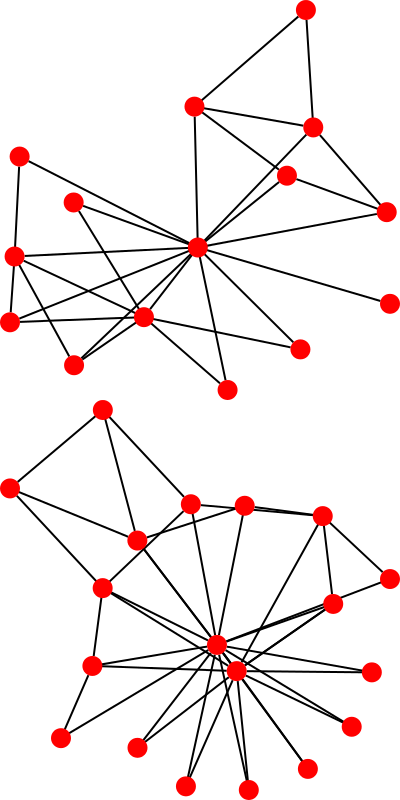
\includegraphics[scale=.32]{2-karate.png}
\end{figure}
\clearpage

\newpage
Q2. We know the group split in two different groups.  Suppose the\\
disagreements in the group were more nuanced -- what would the clubs\\
look like if they split into groups of 3, 4, and 5?\\*

\begin{figure}[H]
  \centering
  \caption{Zachary Karate, Clusters=3, Modularity=0.34878369493754113}
  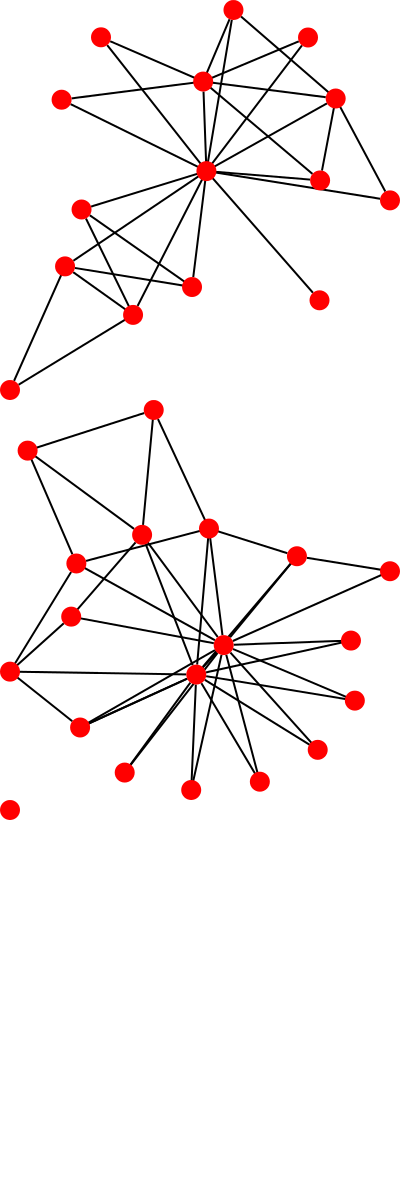
\includegraphics[scale=.32]{3-karate.png}
\end{figure}
\clearpage

\begin{figure}[H]
  \centering
  \caption{Zachary Karate, Clusters=4, Modularity=0.36324786324786335}
  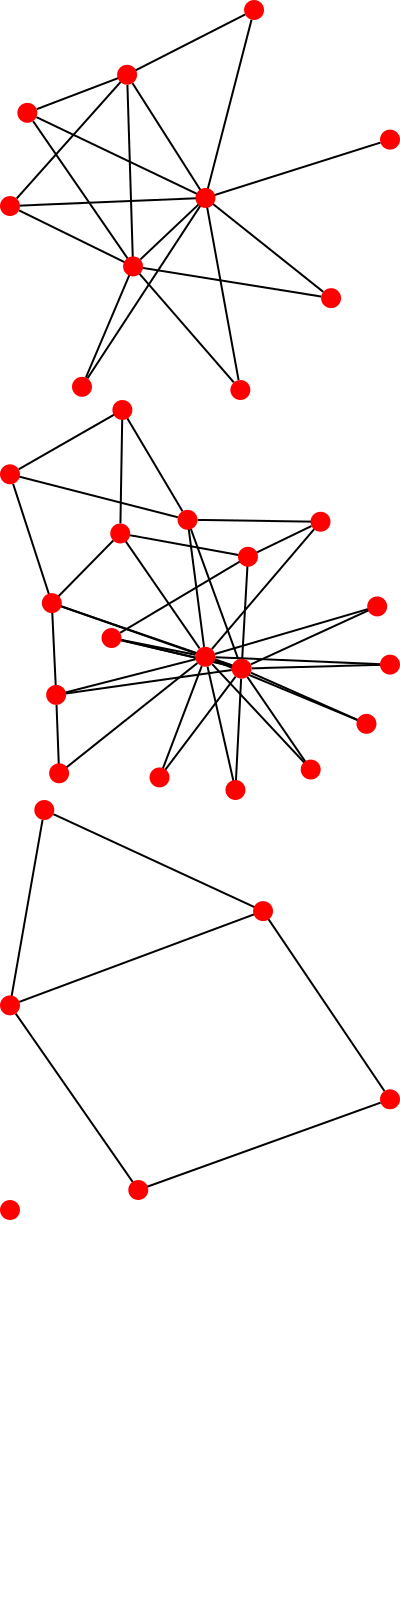
\includegraphics[scale=.25]{4-karate.png}
\end{figure}
\clearpage

\begin{figure}[H]
  \centering
  \caption{Zachary Karate, Clusters=5, Modularity=0.35174227481919795}
  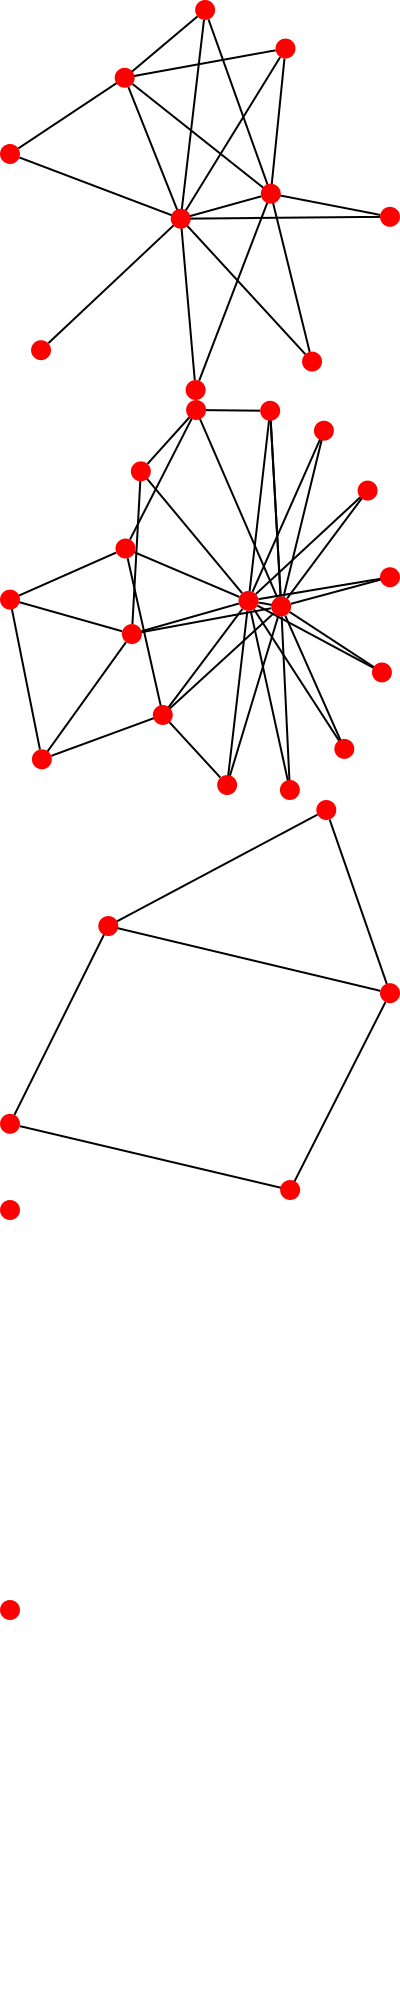
\includegraphics[scale=.2]{5-karate.png}
\end{figure}
\clearpage

\appendix
\newpage
Appendix A
\lstinputlisting[language=python]{calculate.py}

\newpage
Appendix B
\lstinputlisting[language=bash]{imagesAppend}

\end{document}
